\chapter{Определение этногеографической принадлежности}

В данной главе будет рассмотрен вопрос определения этногеографической принадлежности
индивидов на основе STR-маркеров. В контексте данной магистерской диссертации под
этногеографической принадлежностью мы будем понимать задачу отнесения неизвестного
индивида к одному из этногеографических регионов Республики Беларусь: Понеманье (запад),
Западное Полесье (Юго-Запад), Восточное Полесье (Юг), Поднепровье (Восток), Поозерье (Север) и
Центральная Беларусь, рисунок $\left(\ref{image:regions}\right)$. Основной задачей является определение факторов (в данном случае некоторое
множество STR-маркеров), способных дифференцировать популяцию Республики Беларусь. Одной из гиппотез
является возможность разделения индивидов на уровне "Север"/"Юг".


\begin{figure}[h]
\begin{center}
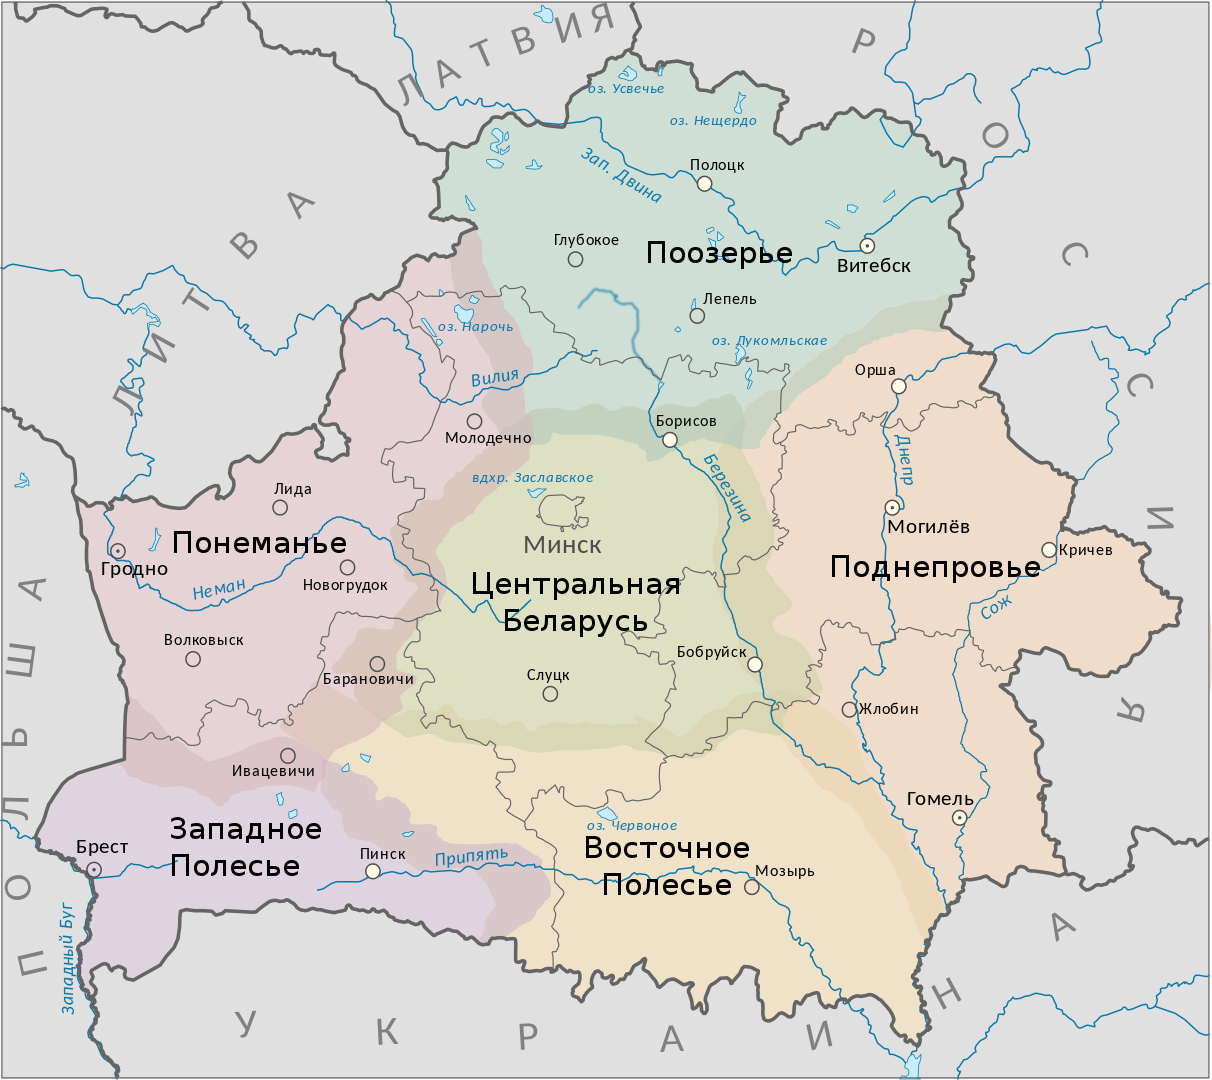
\includegraphics[width=10cm]{images/belarus_regions.png}
\end{center}
  \caption{Энтогеографические регионы Республики Беларусь. Источник}
  \label{image:regions}
\end{figure}

\section{Валидация данных}

\subsection{Данные для проведения экспериментов}

В рамках работы над настоящей магистерской диссертацией был получен доступ к следующим данным:
\begin{itemize}
\item База данных генотипов населения Республики Беларусь, датированная 2018 годом.
Множество локусов включает в себя 13 оригинальных локусов набора CODIS core, а также несколько
других локусов, общим число локусов 18. Общее число записей в полученных данных составляет 830.
Помимо идентификатора генотипа, в данных содержится информация о населенных пунктах индивидов, которым
принадлежат соответствующие генотипы. Также, присутствуют информация об этногеографической
принадлежности соответствующих индивидов. Отметим, что все локусы соответствуют аутосомным хромосомам.

\item Более новая база данных генотипов населения Республики Беларусь, датированная 2020 годом.
В данной базе содержатся генотипы 28 аутосомных локусов, в том числе и оригинальные локусы
набора CODIS core. Общее число доспупных записей - 548.

\item Анкетные данные индивидов, чьи генотипы содержатся в базе 2020 года. Данные включают
в себя описание фенотипов (цвет глаз), национальности, персональной информации
(место работы, дата рождения, профессия), также присутствует информация о этногеорафической принадлежности.

\item Дополнительно, было решено воспользоваться открытой популяционной базой NIST 1036,
включающей в себя информацию о генотипах 1034 индивидов, проживающих на территории
Соединенных штатов Америки. В данной базе представлены индивиды следующих групп:
Европеоидной расы (341 генотип), Латиноамериканцы США (235 генотипов), Азиаты (97 генотипов)
и Афроамериканцы (341 генотип). База содержит аллели 29 локусов. Основной мотивацией для включения
данной базы в рассмотрение послужил следующий вопрос: в какой степени репрезентативны аутосомные
маркеры на основе которых собраны данные генотипах индивидов Республики Беларусь. Позволяют ли они
дифференциировать генотипы хотя бы на уровне рас?
\end{itemize}

\subsection{Оценка корректности информации об этногеорафической принадлежности}

Перед началом работы с данными было принято решение оценить для каждого генотипа
корректность присвоенного этногеорафического региона. Для этого по имеющейся информации
о населенных пунктах для каждого генотипа необходимо было произвести геолокацию, то есть
определить географические координаты. Далее, визуализировав на карте все координаты генотипов
можно было бы оценить качество данных.

Для задачи геолокации было решено использовать библиотеку GeoPy. Библиотека имеет
довольно простой интерфейс, отсутствует ограничение на количество запросов. На практике,
за это пришлось заплатить довольно низким качеством распознавания (в сравнении с
Google Maps API, например), в конечном итоге для некоторых населенных пунктов пришлось узнавать
их координаты мануально.

С целью упрощения и ускорения процесса исправления ошибок, был разработано и реализовано
веб-приложение, позволяющее визуализировать географические координаты генотипов,
редактировать данные (исправление как некорректных координат, полученных в результате
использования библиотеки GeoPy, так и изменять графу "этногеографическая принадлежность"),
а также осуществлять выгрузку исправленных данных. Рисунок $\left(\ref{image:geomapv1}\right)$
демонстрирует часть интерфейса приложения, а также качество исходной разметки. Видно,
что генотипы явно смешаны и в ряде случаев заявленная этногеографическая принадлежность
не соответствует действительности. После анализа данных и исправления разметки,
визуализация координат генотипов имела вид, показанный на рисунке $\left(\ref{image:geomapv2}\right)$.

\begin{figure}[h]
\begin{center}
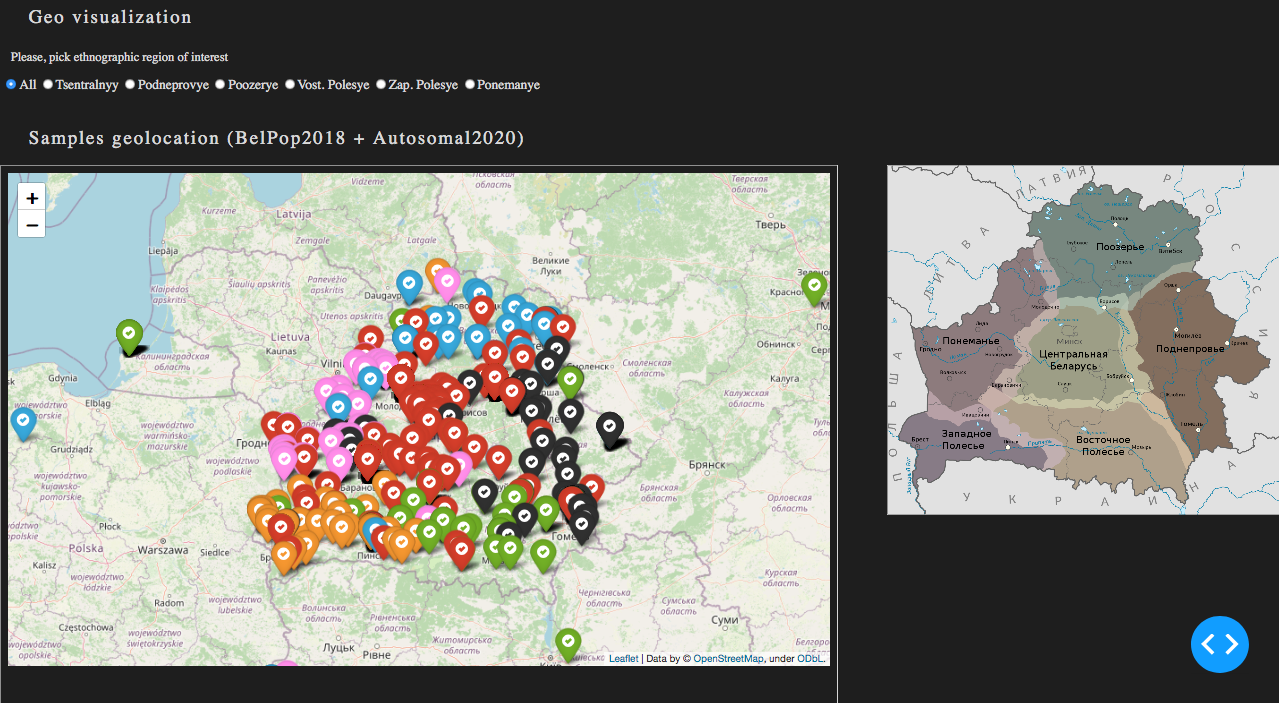
\includegraphics[width=14cm]{images/geomap_v1.png}
\end{center}
  \caption{Часть интерфейса по разметке данных.}
  \label{image:geomapv1}
\end{figure}

\begin{figure}[h]
\begin{center}
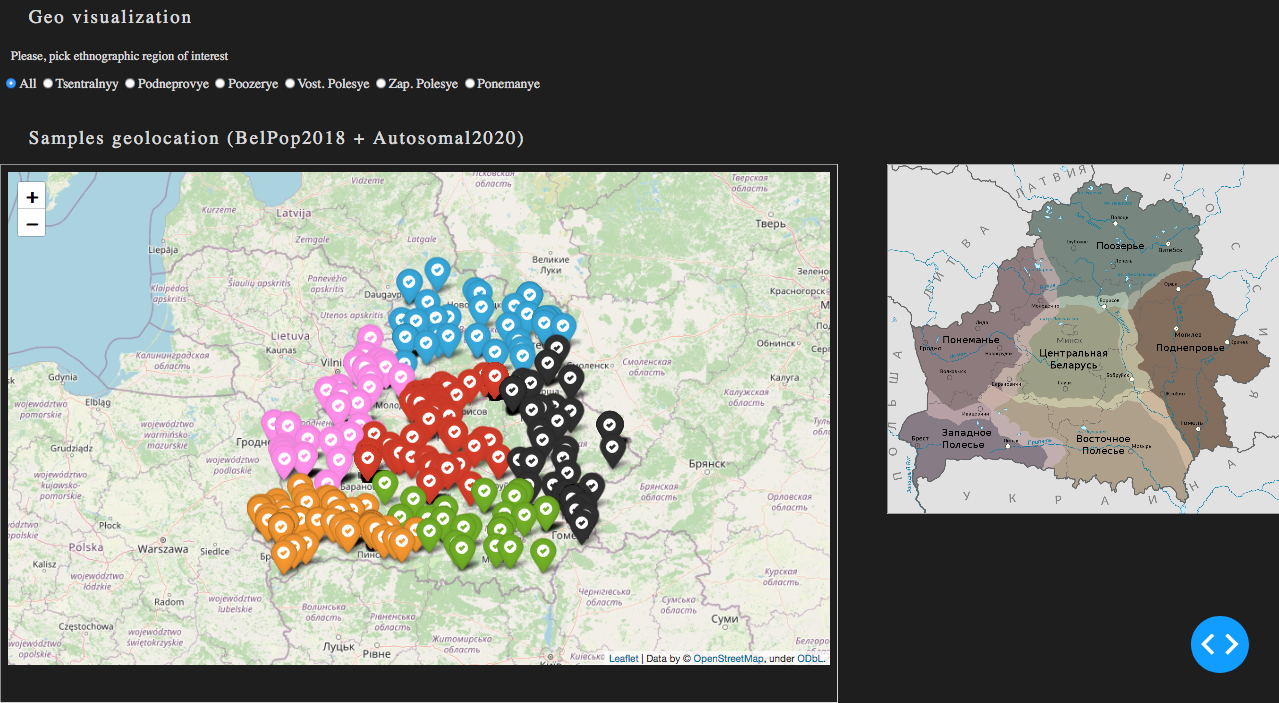
\includegraphics[width=14cm]{images/geomap_v2.png}
\end{center}
  \caption{Визуализация координат генотипов после исправления разметки}
  \label{image:geomapv2}
\end{figure}

\section{Классификация по этногеографическому признаку}

В рамках данного раздела практические эксперименты будут вестись со следующими наборами данных:
\begin{itemize}
\item Объединенная база аутосомных маркеров, состоящая из записей баз генотипов 2018 и 2020 годов.
Результирующая база содержит общие для обоих баз STR-маркеры. Цель объединения - увеличения размера
выборки.

\item Генотипы базы NIST 1036. Анализ генотипов из данной базы не является целью
поставленной в рамках данной магистерской диссертации, однако, сравнительная характеристика
генотипов из данной базы с белорусскими генотипами может быть полезна при анализе дискриминативной
способности имеющихся STR-маркеров.
\end{itemize}

\subsection{Первичный анализ данных}
Одним из базовых инструментов при работе с данными большой размерности является
анализ главных компонент, позволяющий строить проекции данных на меньшее количество размерностей,
тем самым понижая размерность данных. В результате появляется возможность визуализировать данные,
что нередко оказывается полезно, так как позволяет увидеть различного рода зависимости в данных.

Визуализация главных компонент для объединенного набора данных изображена на рисунке $\left(\ref{image:beldata_pca}\right)$.
При более подробном анализе не было выявлено обособленных кластеров, которые бы свидетельствовали
о существовании группы генотипов обладающих какими-либо особыми свойствами, которые отличаются от основной массы.

Анализ главных компонент для генотипов популяции США, рисунок $\left(\ref{image:us_pca}\right)$,
дал более интересные результаты. Можно отчетливо распознать кластер из генотипов афроамериканцев (AA),
а также группу из 3 кластеров, причем каждый кластер содержит генотипы соответствующие определенной
расовой группе. Результат интуитивно понятен с точки зрения различия фенотипов соответствующих
груп генетипов.

Таким образом можно заключить, что имеющиеся STR-маркеры позволяют разделять
генотипы представителей разных рас. В то же время применимость и разделяющая способность данных маркеров
для стратификации на уровне отдельно взятых регионов Республики Беларусь остается под вопросом.

\begin{figure}[h]
\begin{center}
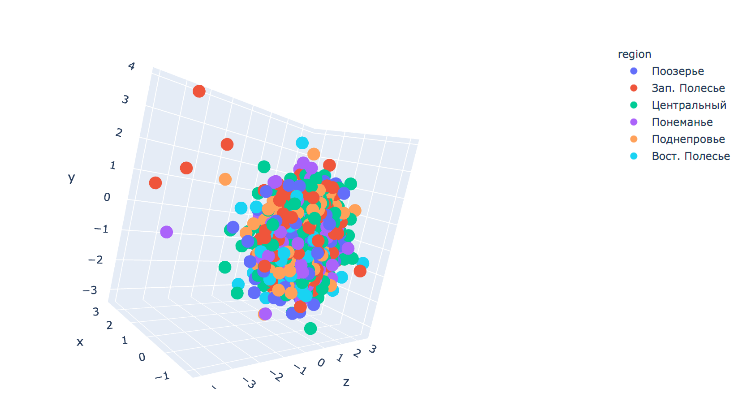
\includegraphics[width=14cm]{images/beldata_pca.png}
\end{center}
  \caption{Визуализация главных компонент объединенного набора белорусских генотипов}
  \label{image:beldata_pca}
\end{figure}

\begin{figure}[h]
\begin{center}
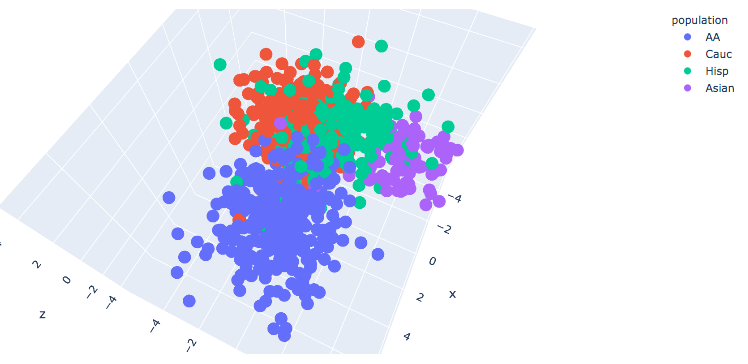
\includegraphics[width=14cm]{images/us_pca.png}
\end{center}
  \caption{Визуализация главных компонент базы генотипов NIST 1036}
  \label{image:us_pca}
\end{figure}

\subsection{Постановка задачи}

Задача классификации этногеорафической принадлежности генотипов может быть сведена
к задаче бинарной классификации. Так, для каждой пары этногеографических регионов будем
стоить отдельную модель, которая для некоторого генотипа будет предсказывать наиболее вероятный
регион. В свою очередь, для конкретной пары регионов $R_{0}$ и $R_{1}$, задача предсказания
одного из регионов может быть сведена к задаче предсказания вероятности принадлежности к одному
из регионов. Тогда, при наличии некоторого порога и некоторой предсказанной вероятности
мы будем иметь возможность сделать выбор в пользу одного из регионов. В общем случае
варьирование порога позволяет делать выбор в пользу каких-либо заранее определенных
ожидаемых свойств построенной модели. Например, мы сможем конролировать отношение ошибок первого
и второго рода. Будем считать, что для заданной пары регионов, каждому примеру можно поставить в соответствие
один из двух классов. Пусть для определенности генотипы меньшего по размеру (с точки зрения
количества примеров в выборке) региона будут соответствовать положительному классу, большего - отрицательному.
Таким образом, для некоторого генотипа нас будет интересовать вероятность его принадлежности
к положительному классу.

При оценке качества классификации довольно часто используются следующие метрики:

\begin{itemize}
\item Точность (англ. precision) - характеризует долю предсказанных объектов положительного класса,
реально относящихся к положительному классу

\item Полнота (англ. recall) - характеризует долю верно предсказанных объектов положительного класса

\item Площадь под кривой точность-полнота (англ. PR AUC). Для некоторого фиксированного классификатора,
при изменении порогового значения точность и полнота предсказаний изменяняются.
Если изобразить значения точности и полноты для различных значений порога, то получим
кривую. При сравнении двух классификаторов, обычно предпочтение отдается классификатору,
для которого площадь под кривой точность-полнота больше. В целом данныя метрика применима
к несбалансированным выборкам, а также, в отличии от ROC кривой, более устойчива для
выборок небольшого размера.
\end{itemize}

Таким образом при оценке качества бинарной классификации будем использовать метрику PR AUC.

\subsection{Описание использованных методов}

Для решения каждой из задач бинарной классификации была использована единая методология.
Далее приводится описание на примере задачи классификации генотипов для двух возможных
этногеорафичесих регионов $R_{0}$ и $R_{1}$ (не теряя общности предположим, что региону $R_{1}$
принадлежит меньшее количество примеров):

\begin{enumerate}
\item Генотипы принадлежащие одному из двух выбранных регионов попадают в общую выборку $X$,
причем, как уже было отмечено выше, каждый генотип относится к положительному либо
негативному классу в соответствии со своим регионом, то есть $y_{i} = \mathbbm{1} \left[ r_{i} == R_{1} \right]$.

\item Выборка $X$ случайным образом разделяется на тренировочную $X_{Train}$ и тестовую $X_{Test}$
в отношении $4:1$. Стандартизация для 2 выборок производится на основе только лишь
тренировочной выборки $X_{Train}$.

\item Тренировочная выборка $X_{Train}$, в свою очередь, делится на тренировочную $X_{train}$ и
валидационную $X_{val}$.

\item Для ряда моделей машинного обучение производится подбор гиперпараметров на тренировочной выборке
$X_{train}$ с количеством фолдов $k=5$. Описание моделей и сеток гиперпараметров приведено ниже.

\item Для каждой модели с подобранными гиперпараметрами производится оценка качества классификации
на валидационной выборке $X_{val}$. Модель, показавшую наибольшее значеие по метрике PR AUC на валидационной
выборке, обозначим как $M_{best}$. При известном наборе оптимальных гиперпараметров производится обучение
модели $M_{best}$ на всей тренировочной выборке $X_{Train}$.

\item Модель $M_{best}$ признается лучшей (так называемый отбор моделей
(англ. model selection)), и ее качество классификации оценивается на тестовой выборке $X_{Test}$.
Значение метрики PR AUC на тестовой выборке $X_{Test}$ принимается за итоговое качество классификации
для двух выбранных этногеорафичесих регионов $R_{0}$ и $R_{1}$.

\end{enumerate}

Для решения задач бинарной классификации были использованы следующие модели машинного обучения:
\begin{itemize}
\item Случайный лес (англ. random forest) в реализации библиотеки scikit-learn.
По описанной выше схеме осуществлялся подбор следующих гиперпараметров: количество деревьев, доля признаков
для построения каждого дерева, максимальная глубина деревьев, минимальное количество примеров в листах,
минимальное количство примеров для разбиения внутренних вершин.

\item Логистическая регрессия (англ. logistic regression) в реализации библиотеки scikit-learn.
Подбор осуществлялся для следующих гиперпараметров: параметр и вид нормы регуляризации.

\item Метод опорных векторов (англ. support vector machines) в реализации библиотеки scikit-learn.
Подбор осуществлялся для следующих гиперпараметров: параметр регуляризации, вид ядра, а также степень
в случае полиномиального типа ядра - степень.


\item Градиентный бустинг (англ. gradient boosting) в реализации библиотеки CatBoost.
Подбор осуществлялся для следующих гиперпараметров: глубина деревьев, скорость обучения и
параметры для регуляризации.
\end{itemize}

\subsection{Результаты}

Для всех возможных пар этногеографических регионов были проведены эксперименты с целью установления
качества бинарной классификации генотипов. Сводная таблица с результатами приведена на рисунке
$\left(\ref{image:bel_pr}\right)$. На основании абсолютных значений выбранной метрики можно отметить
хорошее качество классификации для пары регионов Понеманье-Поозерье. Основываясь же на относительных значениях,
можно выделить регион Понеманье, имеющий неплохие показатели в контексте разделимости с
остальными этногеографическими регионами (за исключением Центрального). Также стоит отметить регион
Западное Полесье, а именно результаты классификации с регионами Поозерье и Понеманье.

Дополнительно были проведены эксперименты с генотипами популяций США базы NIST 1036.
Результаты приведены на рисунке $\left(\ref{image:bel_us_pr}\right)$. Высокое качество
классификации между популяциями США подтверждают выводы сделанные на основе анализа
главных компонент. Также, стоит отметить относительно низкое качество между
белорусскими генотипами и генотипами Европиоидной расы индивидов из США.
Данный результат отчасти оправдывает невысокое качество классификации белорусских генотипов
в контексте задачи определения этногеографической принадлежности.

\begin{figure}[h]
\begin{center}
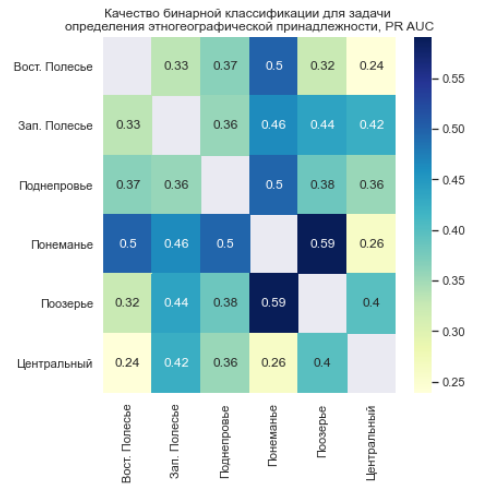
\includegraphics[width=8cm]{images/bel_reg_pr_auc.png}
\end{center}
  \caption{Качество классификации белорусских генотипов (на уровне этногеорафичесих регионов)}
  \label{image:bel_pr}
\end{figure}

\begin{figure}[h]
\begin{center}
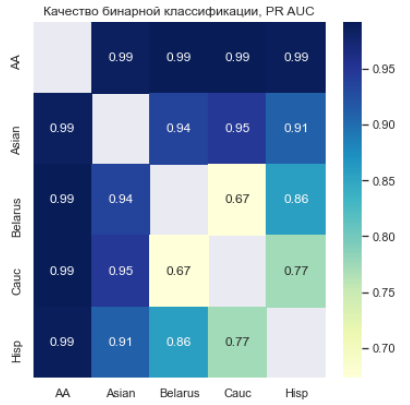
\includegraphics[width=8cm]{images/bel_us_pr.png}
\end{center}
  \caption{Качество классификации белорусских генотипов и генотипов популяций США}
  \label{image:bel_us_pr}
\end{figure}

\section{Выводы}

В результате практических экспериментов были получены следующие результаты:
\begin{itemize}
\item Имеющийся набор STR-маркеров и генотипы она его основе обладают достаточной вариабельностью аллелей
для обучения моделей машинного обучения с целью классификации расы индивида на основе генотипа.

\item Проведена оценка качества классификации генотипов с целью определения этногеографической принадлежности

\item Основываясь на полученных результатах классификации, можно выделить этногеографические регионы
Понеманье и Западное Полесье, ввиду относительно высокой степени отличия их от остальных регионов.
\end{itemize}
